\documentclass[review,3p,times]{elsarticle}

\usepackage{amsmath}
\usepackage{amssymb}
\usepackage{graphicx}
\graphicspath{{figures/}}
\usepackage{booktabs}
\usepackage{hyperref}
\usepackage{microtype}
\usepackage{siunitx}
\usepackage{subcaption}
\usepackage{cleveref}
\usepackage{url}

\journal{Optics and Lasers in Engineering}

\begin{document}

\begin{frontmatter}

\title{Grouped and Frequency-Controlled Audits of Frozen ESPI Representations for Full-Field Vibration Pattern Analysis}

\author[inst1]{[Author Names / ESPI Team]}
\affiliation[inst1]{organization={[Department Name, Institution Name]},
            addressline={[Address Line]}, 
            city={[City]},
            postcode={[Postcode]}, 
            state={[State]},
            country={[Country]}}

\begin{abstract}
Electronic speckle pattern interferometry (ESPI) provides full-field optical measurements of vibration patterns, but classification accuracy alone does not demonstrate that a model has learned reusable ESPI representations. This study presents a representation audit of frozen image-derived embeddings for five-class ESPI modal-pattern recognition under grouped board and material evaluation protocols. We compare random, ImageNet-pretrained, and two ESPI-trained residual encoders (v6.1 and distribution-aware v6.2-A). Frequency-only metadata controls outperform image-derived embeddings globally, demonstrating that the current label protocol is strongly frequency-dominated. However, under matched grouped evaluation, v6.2-A emerges as the strongest image-derived frozen ESPI encoder baseline, achieving 93.56\% Board LOBO and 93.49\% Material LOMO Macro-F1 at fixed $k=10$. A targeted frequency-overlap and geometry analysis shows that v6.2-A embeddings provide complementary morphology information in frequency-ambiguous modes, and exhibit tighter intra-class representation geometry. The results support v6.2-A as the strongest evaluated image-derived frozen ESPI representation, while establishing scalar frequency as the dominant metadata-only predictor. Acoustic-response prediction, learned spectral modules, and full physics-aligned encoder validation remain outside the present scope.
\end{abstract}

\begin{keyword}
Electronic speckle pattern interferometry \sep Representation learning \sep Vibration pattern analysis \sep Specimen-invariance \sep Information budget
\end{keyword}

\end{frontmatter}

\section{Introduction}
\label{sec:intro}

Electronic speckle pattern interferometry (ESPI) is a full-field optical metrology technique for measuring displacement and vibration-induced surface deformation through coherent speckle interference [1,2]. In vibration studies, ESPI fringe and speckle patterns encode spatially distributed modal information that is not available from a single point sensor. These full-field interferometric images are therefore attractive for automated modal-pattern recognition, but they also contain signatures associated with board geometry, material, acquisition condition, and excitation frequency.

In ESPI vibration measurements, fringe density, nodal-line organization, and spatial modulation patterns are linked to the underlying deformation field and modal response of the specimen. A reusable ESPI representation should therefore preserve full-field modal morphology rather than only reproduce label correlations under a random split.

Most supervised ESPI classification studies evaluate whether a trained model assigns each image to the correct modal class on a validation split. This is a necessary baseline, but it addresses only the final classification decision. It does not determine whether the internal feature space is reusable as an ESPI representation. A classifier head may separate classes under a stratified split while the corresponding embedding space remains strongly tied to board-, material-, frequency-, or acquisition-specific correlations.

This manuscript evaluates ESPI models as frozen encoder candidates. Encoder weights remain fixed, and the saved representations are tested with lightweight downstream heads: fixed-k kNN, prototype classification, and balanced logistic-regression linear probes. This approach separates representation geometry from the original classifier head and provides an audit of whether the embedding space remains informative under grouped evaluation.

Grouped evaluation is important for optical metrology applications because a reusable ESPI representation should remain useful when measurements come from boards or materials not present in the reference set. We therefore include board-held-out and material-held-out protocols. In the board-grouped evaluation, the reference set excludes the held-out board. In the material-grouped evaluation, the reference set excludes the held-out material. These tests are frozen-embedding grouped evaluations, not retrained CNN LOBO/LOMO experiments.

The five modal labels are also frequency-structured. Consequently, \texttt{frequency\_hz} must be treated as an information-budget control. Without a frequency-only baseline, high modal-label accuracy could be mistaken for evidence that image morphology alone explains the label structure. This study therefore separates metadata-only predictability from image-derived frozen representation evidence. Acoustic-response prediction is treated as future validation rather than a current result.

The evaluation covers generic, ESPI-specific, physics-aware, and metadata-controlled sources. Random ResNet-18 and ImageNet-pretrained ResNet-18 embeddings serve as generic visual controls. v6.1 is the reference ESPI-specific baseline. v6.2-A is the primary ESPI-trained image-derived baseline evaluated in this study. Hierarchical v6.2 phase2 is included as a controlled physics-aware architectural comparison. Frequency-only and frequency-plus-embedding controls quantify how much modal-label information is carried by excitation frequency.

The main finding is a controlled trade-off. Under fixed $k=10$, v6.1 is slightly stronger than v6.2-A in stratified kNN evaluation (93.65\% versus 92.78\% Macro-F1). Under grouped fixed $k=10$ evaluation, v6.2-A is strongest among image-derived frozen encoders, reaching 93.56\% Board LOBO Macro-F1 and 93.49\% Material LOMO Macro-F1. Frequency-only controls are stronger overall for the current label protocol, reaching 98.67\%, 97.49\%, and 94.09\% Macro-F1 under stratified, Board LOBO, and Material LOMO protocols. The appropriate claim is therefore precise: v6.2-A is the strongest image-derived frozen ESPI encoder baseline among the evaluated encoders, while \texttt{frequency\_hz} is the dominant metadata-only predictor for the current five-class modal-label protocol.

The present study establishes frozen image-derived ESPI representation evidence under fixed grouped evaluation protocols. The present scope is restricted to frozen image-derived ESPI representation auditing; acoustic-response prediction, learned spectral modules, and full physics-aligned encoder validation define subsequent validation stages.

\subsection{Contributions}
\subsection{Contributions}
\begin{itemize}
    \item \textbf{Frozen ESPI encoder audit protocol.} We define a representation-level audit for ESPI embeddings using fixed $k=10$ kNN, diagnostic best-k sensitivity analysis, prototype classification, linear probes, board-grouped testing, material-grouped testing, class-level metrics, and zero-recall diagnostics.
    \item \textbf{Controlled baseline and metadata comparison.} We evaluate Random ResNet-18, ImageNet ResNet-18, v6.1, v6.2-A, and hierarchical v6.2 phase2 embeddings, and add frequency-only and frequency-plus-embedding controls within a common normalized schema.
    \item \textbf{Grouped image-derived robustness result.} We show that v6.2-A is the strongest grouped-robust image-derived frozen ESPI encoder baseline, while v6.1 remains slightly stronger under fixed $k=10$ stratified kNN and frequency metadata remains stronger for the current label task.
    \item \textbf{Per-class and fold-level stability analysis.} We show that v6.2-A improves grouped F1 over v6.1 across all five modal classes and wins 5/6 board folds and 2/2 material folds. We demonstrate that this advantage persists under strict class--material--frequency-matched balanced subset evaluation.
    \item \textbf{Dimension-matched PCA and targeted overlap analyses.} We show that the v6.2-A robustness advantage is structural rather than a dimensional confound, and that image-derived spatial morphology resolves frequency ambiguity in the localized \texttt{1\_2} and \texttt{2\_1} overlap region.
    \item \textbf{Quantitative embedding geometry.} We quantify frozen-embedding geometry, showing that v6.2-A produces tighter intra-class clusters and stronger between-class separation than v6.1.
\end{itemize}

\section{Related Work}
\label{sec:related}

\subsection{Full-field ESPI Vibration Metrology}
Electronic speckle pattern interferometry is a full-field optical metrology technique for measuring displacement and vibration-induced surface deformation through coherent speckle interference [1,2]. In vibration studies, ESPI fringe patterns encode spatially distributed modal information rather than isolated point measurements, which makes them well suited for mode-shape inspection, nondestructive testing, and specimen-level comparison. This full-field structure also creates a representation-learning question: a classifier may separate labels under a conventional split without necessarily producing image-derived embeddings that remain stable across boards, materials, or acquisition conditions. The present work therefore uses ESPI classification as the experimental context, but evaluates frozen representation quality under grouped board/material protocols.

\subsection{Fringe, Phase, and Spectral Analysis}
Classical interferometric analysis relies heavily on fringe, phase, and spectral structure. Fourier-transform fringe analysis provides a standard route from fringe patterns to phase-related quantities [3], while two-dimensional phase unwrapping methods address the recovery of continuous phase fields from wrapped measurements [4]. Speckle optics also motivates frequency-domain descriptions of spatial interference patterns [5]. These ideas motivate the deterministic spectral descriptors used here as supplementary controls. The descriptors summarize FFT energy distributions and anisotropy, but they are not a trained LeFFT model and are not used to claim LeFFT superiority. Recent deep learning approaches have explored neural networks for ESPI fringe denoising [9], phase retrieval [10], and continuous phase unwrapping [12], confirming the ongoing shift from analytical to learned interferometric analysis [11, 13]. Our study complements this shift by focusing on representation and frozen-feature evaluation [14].

\subsection{CNN Representations and Frozen Encoder Evaluation}
Residual convolutional networks provide a standard backbone family for visual representation learning [6], and ImageNet pretraining is widely used as a generic visual baseline [7]. In optical metrology, however, strong classification accuracy does not by itself establish reusable representation quality. Frozen-embedding audits using kNN, prototype classifiers, and linear probes provide a lightweight way to test whether the embedding space itself carries class-relevant structure, rather than relying only on the final classifier head. This distinction is central to the present comparison between generic ResNet controls, ESPI-specific v6.1 and v6.2-A embeddings, and the hierarchical v6.2 phase2 branch.

\subsection{Grouped Evaluation and Distribution-shift Controls}
Grouped evaluation is important when samples share specimen, acquisition, or material structure. Stratified splits can overestimate robustness if training and validation sets contain closely related samples from the same physical boards or materials. Domain-generalization benchmarks similarly emphasize that model selection and evaluation should respect group structure when the intended use involves distribution shift [8]. The board-held-out and material-held-out protocols used here are therefore treated as grouped evaluation tests for frozen ESPI representations. Material LOMO is interpreted descriptively as a material-held-out stress test because only two material groups are available.

\subsection{Frequency Metadata and Information-budget Controls}
Modal labels in this dataset are strongly frequency-structured, so frequency metadata is a necessary information-budget control. A model that predicts labels from \texttt{frequency\_hz} alone does not demonstrate image-derived ESPI representation quality, but it does define how much label information is available outside the image. The present study therefore reports frequency-only and frequency-fusion controls alongside image-derived frozen embeddings. This framing keeps the main claim specific: v6.2-A is evaluated as an image-derived frozen ESPI encoder baseline, while frequency metadata is treated as a dominant metadata-only predictor for the current label protocol.

\section{Methods}
\label{sec:methods}

\subsection{Dataset and Task Definition}
The dataset contains ESPI full-field vibration patterns organized under a five-class modal protocol. Each sample belongs to one of five modal labels: \texttt{1\_1H}, \texttt{1\_1T}, \texttt{1\_2}, \texttt{2\_1}, or \texttt{higher}.

The frozen-encoder evidence set contains 12,944 samples from six boards (\texttt{C01}, \texttt{C02}, \texttt{C03}, \texttt{W01}, \texttt{W02}, \texttt{W03}) and two materials (\texttt{carbon}, \texttt{wood}). All boards and both materials contain all five modal classes. No board- or material-held-out fold lacks held-out or reference classes, so grouped Macro-F1 values are not artifacts of missing-class folds.

The class distribution is strongly imbalanced. The \texttt{higher} class contains 10,115 samples, corresponding to 78.14\% of the dataset. The remaining classes contain 653 samples for \texttt{1\_1H}, 669 samples for \texttt{1\_1T}, 738 samples for \texttt{1\_2}, and 769 samples for \texttt{2\_1} (see Supplementary Table S1 for details).

Macro-F1 is used as a primary summary metric because the dataset is class-imbalanced. Accuracy can be dominated by the majority \texttt{higher} class, whereas Macro-F1 gives equal weight to each modal class. This is necessary for assessing minority modal classes under grouped evaluation.

\begin{figure}[tbp]
\centering
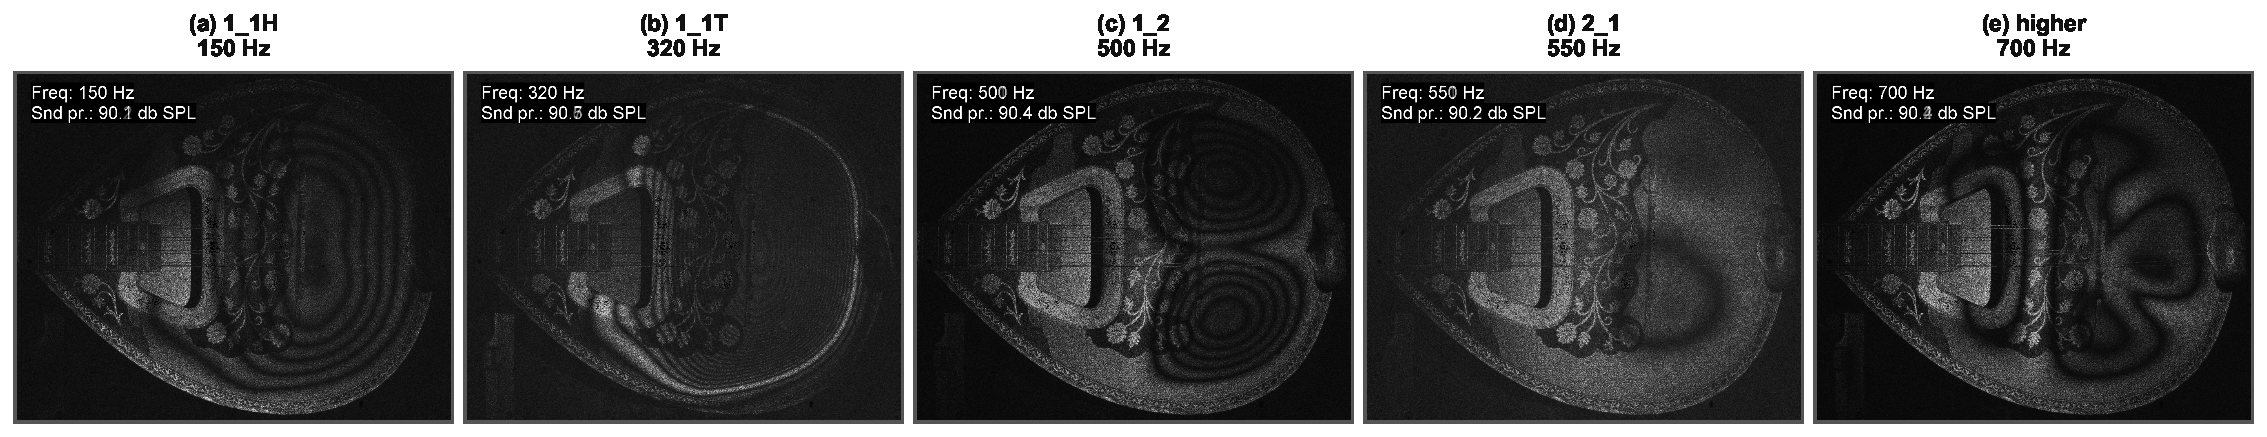
\includegraphics[width=\textwidth]{Figure_1_Representative_Patterns}
\caption{Representative ESPI vibration patterns for the five modal labels: (a) Mode 1\_1H (Fundamental Horizontal, 150 Hz), (b) Mode 1\_1T (Fundamental Torsional, 320 Hz), (c) Mode 1\_2 (Two-axial Bending, 500 Hz), (d) Mode 2\_1 (Complex Torsional, 550 Hz), and (e) Mode higher (High-frequency fringe density, 700 Hz), recorded on board W01 (wood). The progression illustrates the correlation between increasing excitation frequency and the complexity/density of the interferometric fringes, which grounds the representation analysis in structural mechanics.}
\label{fig:fig1}
\end{figure}

\subsection{Encoder Sources}
Five frozen representation sources are evaluated.
The \textbf{Random ResNet-18} baseline is an untrained generic visual control. It tests whether architectural texture bias alone can produce apparent stratified separability.
The \textbf{ImageNet ResNet-18} baseline is a generic pretrained control. ESPI images are passed through an ImageNet-pretrained ResNet-18 feature extractor, and embeddings are taken from the pre-classifier average-pooling representation.
\textbf{v6.1} is the reference ESPI-specific baseline. It uses a one-channel ESPI input, a frozen ResNet18-style backbone, and a lightweight classifier head. It does not include an explicit Fourier, phase, or physics branch.
\textbf{v6.2-A} is the official reportable ESPI baseline and the main image-derived frozen encoder candidate. It is based on the v6.1 architecture and remains a conservative ResNet18-style model rather than a LeFFT-based or hierarchical physics-aware architecture. Its training configuration includes distribution-aware/domain-mixed sampling logic, clean/averaged/pseudo-noisy batch composition, targeted noisy-like augmentation, class-imbalance handling, and zero-recall safeguards.
The \textbf{hierarchical v6.2 phase2} branch is included as a controlled physics-aware architectural comparison. It contains denoising, a learnable Fourier-prior / LeFTP path, wrapped/unwrapped phase and amplitude outputs, multiscale physics features, a gatekeeper head, an expert embedding, and an ArcFace head.

\subsection{Frozen Embedding Extraction}
All comparisons use frozen embeddings. Encoder weights are not updated, and no deep model is retrained or fine-tuned. Lightweight evaluation heads are fitted only on the relevant training/reference fold.

For v6.1, the extraction report documents a clean checkpoint load audit with 124 matched keys, 0 missing keys, 0 unexpected keys, and 0 shape mismatches. The full extraction produced 12,944 embeddings of shape $[12944, 512]$, with 0 NaN values, 0 Inf values, 0 duplicate paths, and nonzero variance.
For the Random and ImageNet ResNet-18 controls, ESPI images were loaded as grayscale and resized to $256 \times 256$. Both baselines produced 12,944 embeddings of dimension 512 with 0 NaN values, 0 Inf values, 0 duplicate paths, and nonzero variance.

\subsection{Normalized Feature Schema}
All feature dumps were normalized to a common NPZ schema before unified evaluation. The schema stores embeddings, labels, label names, paths, board identifiers, material identifiers, frequency metadata, split labels, split-group identifiers, distribution groups, checkpoint metadata, embedding point, model name, source feature identifier, and schema version. The v6.2-A normalized feature dump contains 12,944 samples and 1280-dimensional embeddings. The hierarchical v6.2 phase2 normalized feature dump contains 12,944 samples and 512-dimensional embeddings.

\subsection{Evaluation Protocol}
The primary kNN protocol uses cosine kNN with fixed $k=10$. This value was locked as the development/default grouped kNN setting before manuscript hardening and is used for the main grouped Board LOBO and Material LOMO claims. Additional stratified kNN values for $k = 1, 3, 5, 10, 20$ are reported only as diagnostic sensitivity analysis. Best-k results are not used as the primary manuscript protocol.

All feature scaling, standardization, or normalization used by lightweight heads is fitted only on the training/reference fold and then applied to the held-out fold. Grouped held-out samples are not used to fit preprocessing. This rule applies to stratified train/validation evaluation, board-grouped evaluation, material-grouped evaluation, frequency-only controls, frequency-fusion controls, and deterministic spectral descriptor controls.

The prototype classifier computes one class prototype per class from the reference fold and assigns each test embedding to the nearest prototype. The linear probe uses balanced logistic regression with maximum iterations set to 5000.

The board-grouped protocol holds out each board as the test group and uses all other boards as the reference group. The material-grouped protocol holds out each material group and uses the other material group as the reference group. Grouped Board LOBO and Material LOMO scores are reported as arithmetic means of held-out-group Macro-F1 values, not as pooled predictions across all held-out samples. 95\% bootstrap confidence intervals for the main summary Macro-F1 metrics were computed using 200 iterations.

\subsection{Frequency-only, Fusion, and Spectral Descriptor Controls}
Frequency-only controls use \texttt{frequency\_hz} as the sole input feature. We evaluated balanced logistic regression and random forest under the same stratified, board-grouped, and material-grouped protocols. Frequency-plus-embedding fusion concatenates scalar \texttt{frequency\_hz} with frozen encoder embeddings.

We also evaluated deterministic spectral / LeFFT-inspired descriptors as a lightweight supplementary control. These descriptors are computed from grayscale ESPI images using deterministic FFT-based statistics; they are not a trained LeFFT model. No frequency-control or spectral-control experiment updates encoder weights, trains a deep model, implements acoustic-response prediction, or supports a LeFFT superiority claim.

\subsection{Class-Level Diagnostics and QA}
Class-level diagnostics determine whether grouped robustness is distributed across modal classes or driven mainly by the majority class. The diagnostics include per-class precision, recall, F1, support, macro averages, weighted averages, confusion matrices, zero-recall rows, per-board class diagnostics, and per-material class diagnostics.

\subsection{Dimension-Matched PCA Control}
To ensure that performance differences are not an artifact of varying embedding capacities, we evaluated the representation under dimensionality reduction. A fold-local Principal Component Analysis (PCA) was fitted exclusively on each training/reference fold and applied to the corresponding held-out fold to project embeddings down to 512, 256, and 128 dimensions.

\subsection{Frequency-Overlap Pair Analysis}
To evaluate image-derived complementary information when scalar frequency becomes weakly discriminative, we isolated the structurally similar \texttt{1\_2} and \texttt{2\_1} modal classes. The analysis used the full binary subset ($N=1{,}507$) and a strictly restricted overlap interval from 550.00 to 556.00 Hz ($N=43$), comparing frequency-only performance to frequency-plus-embedding fusion.

\subsection{Balanced Subset Construction}
To test whether robustness is driven by class imbalance or frequency-distribution artifacts, we constructed three balanced evaluation subsets: class-balanced, class--material-balanced, and class--material--frequency-matched. The strictest frequency-matched subset paired \texttt{wood} and \texttt{carbon} samples within 25 Hz frequency bins inside each modal class and applied a final class-level min-cell balancing, yielding 184 samples per class and a total $N=920$.

\subsection{Quantitative Embedding Geometry}
We quantified frozen-embedding geometry directly, independently of downstream classifier metrics. The evaluated metrics include the cosine Silhouette score, the Davies--Bouldin index, the intra/inter-class cosine distance ratio, and the cross-board/cross-material same-class nearest-neighbor consistency.

\section{Results}
\label{sec:results}

\subsection{Encoder Baseline Overview}
The unified evaluation compares five image-derived frozen representation sources under the same fixed $k=10$ protocol and grouped evaluation design (\cref{tab:table1}, with a visual summary across protocols in \cref{fig:central_comparison}). The generic Random and ImageNet ResNet-18 controls achieve non-trivial stratified scores but fail under grouped board/material testing. v6.1 is the strongest fixed-k stratified image-derived baseline, while v6.2-A is the strongest grouped image-derived baseline. Hierarchical v6.2 phase2 is technically valid but not competitive in frozen embedding evaluation.

\begin{figure}[tbp]
\centering
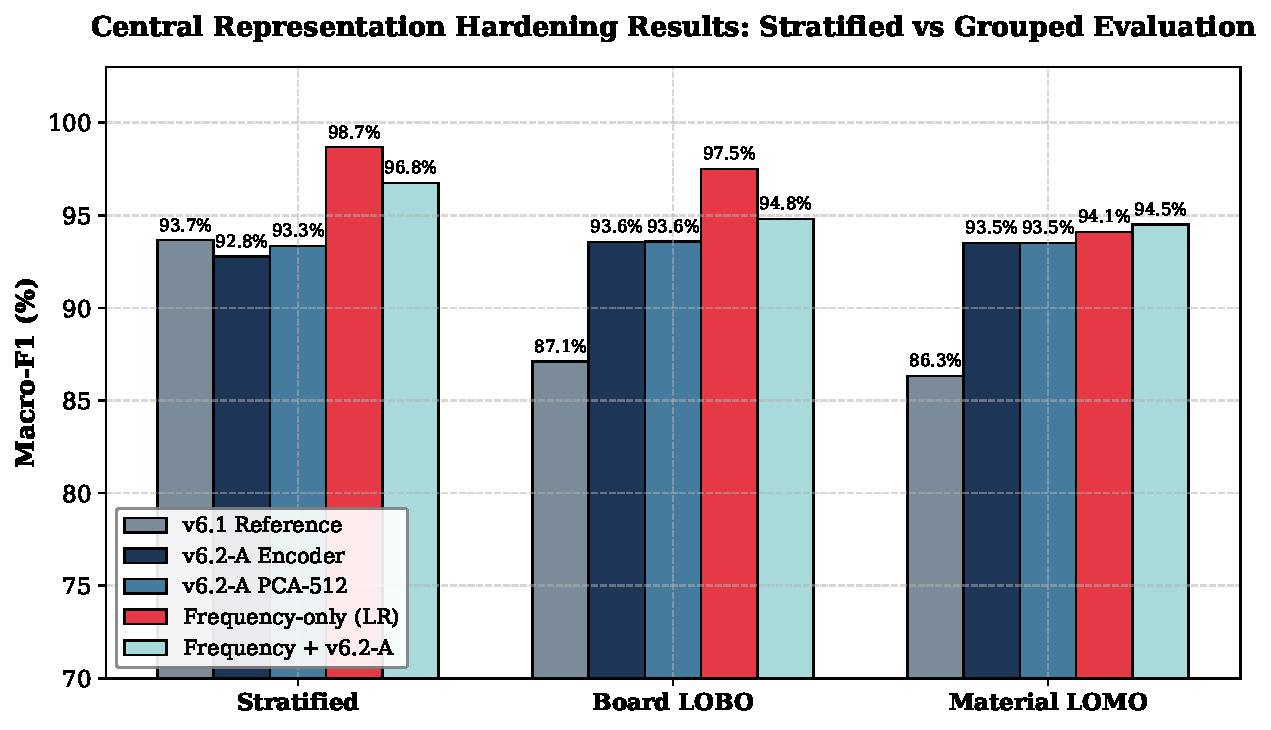
\includegraphics[width=0.9\textwidth]{central_result_comparison}
\caption{Comparison of Macro-F1 classification performance across evaluation protocols for v6.1 baseline, v6.2-A frozen encoder, v6.2-A PCA-512 dimension-matched control, frequency-only baseline, and frequency + v6.2-A fusion. The panel summarizes performance under (a) stratified, (b) grouped board-held-out (Board LOBO), and (c) grouped material-held-out (Material LOMO) protocols, demonstrating the grouped robustness of the v6.2-A representation and the localized complementary gains of fusion over the frequency-only control.}
\label{fig:central_comparison}
\end{figure}

\begin{figure}[tbp]
\centering
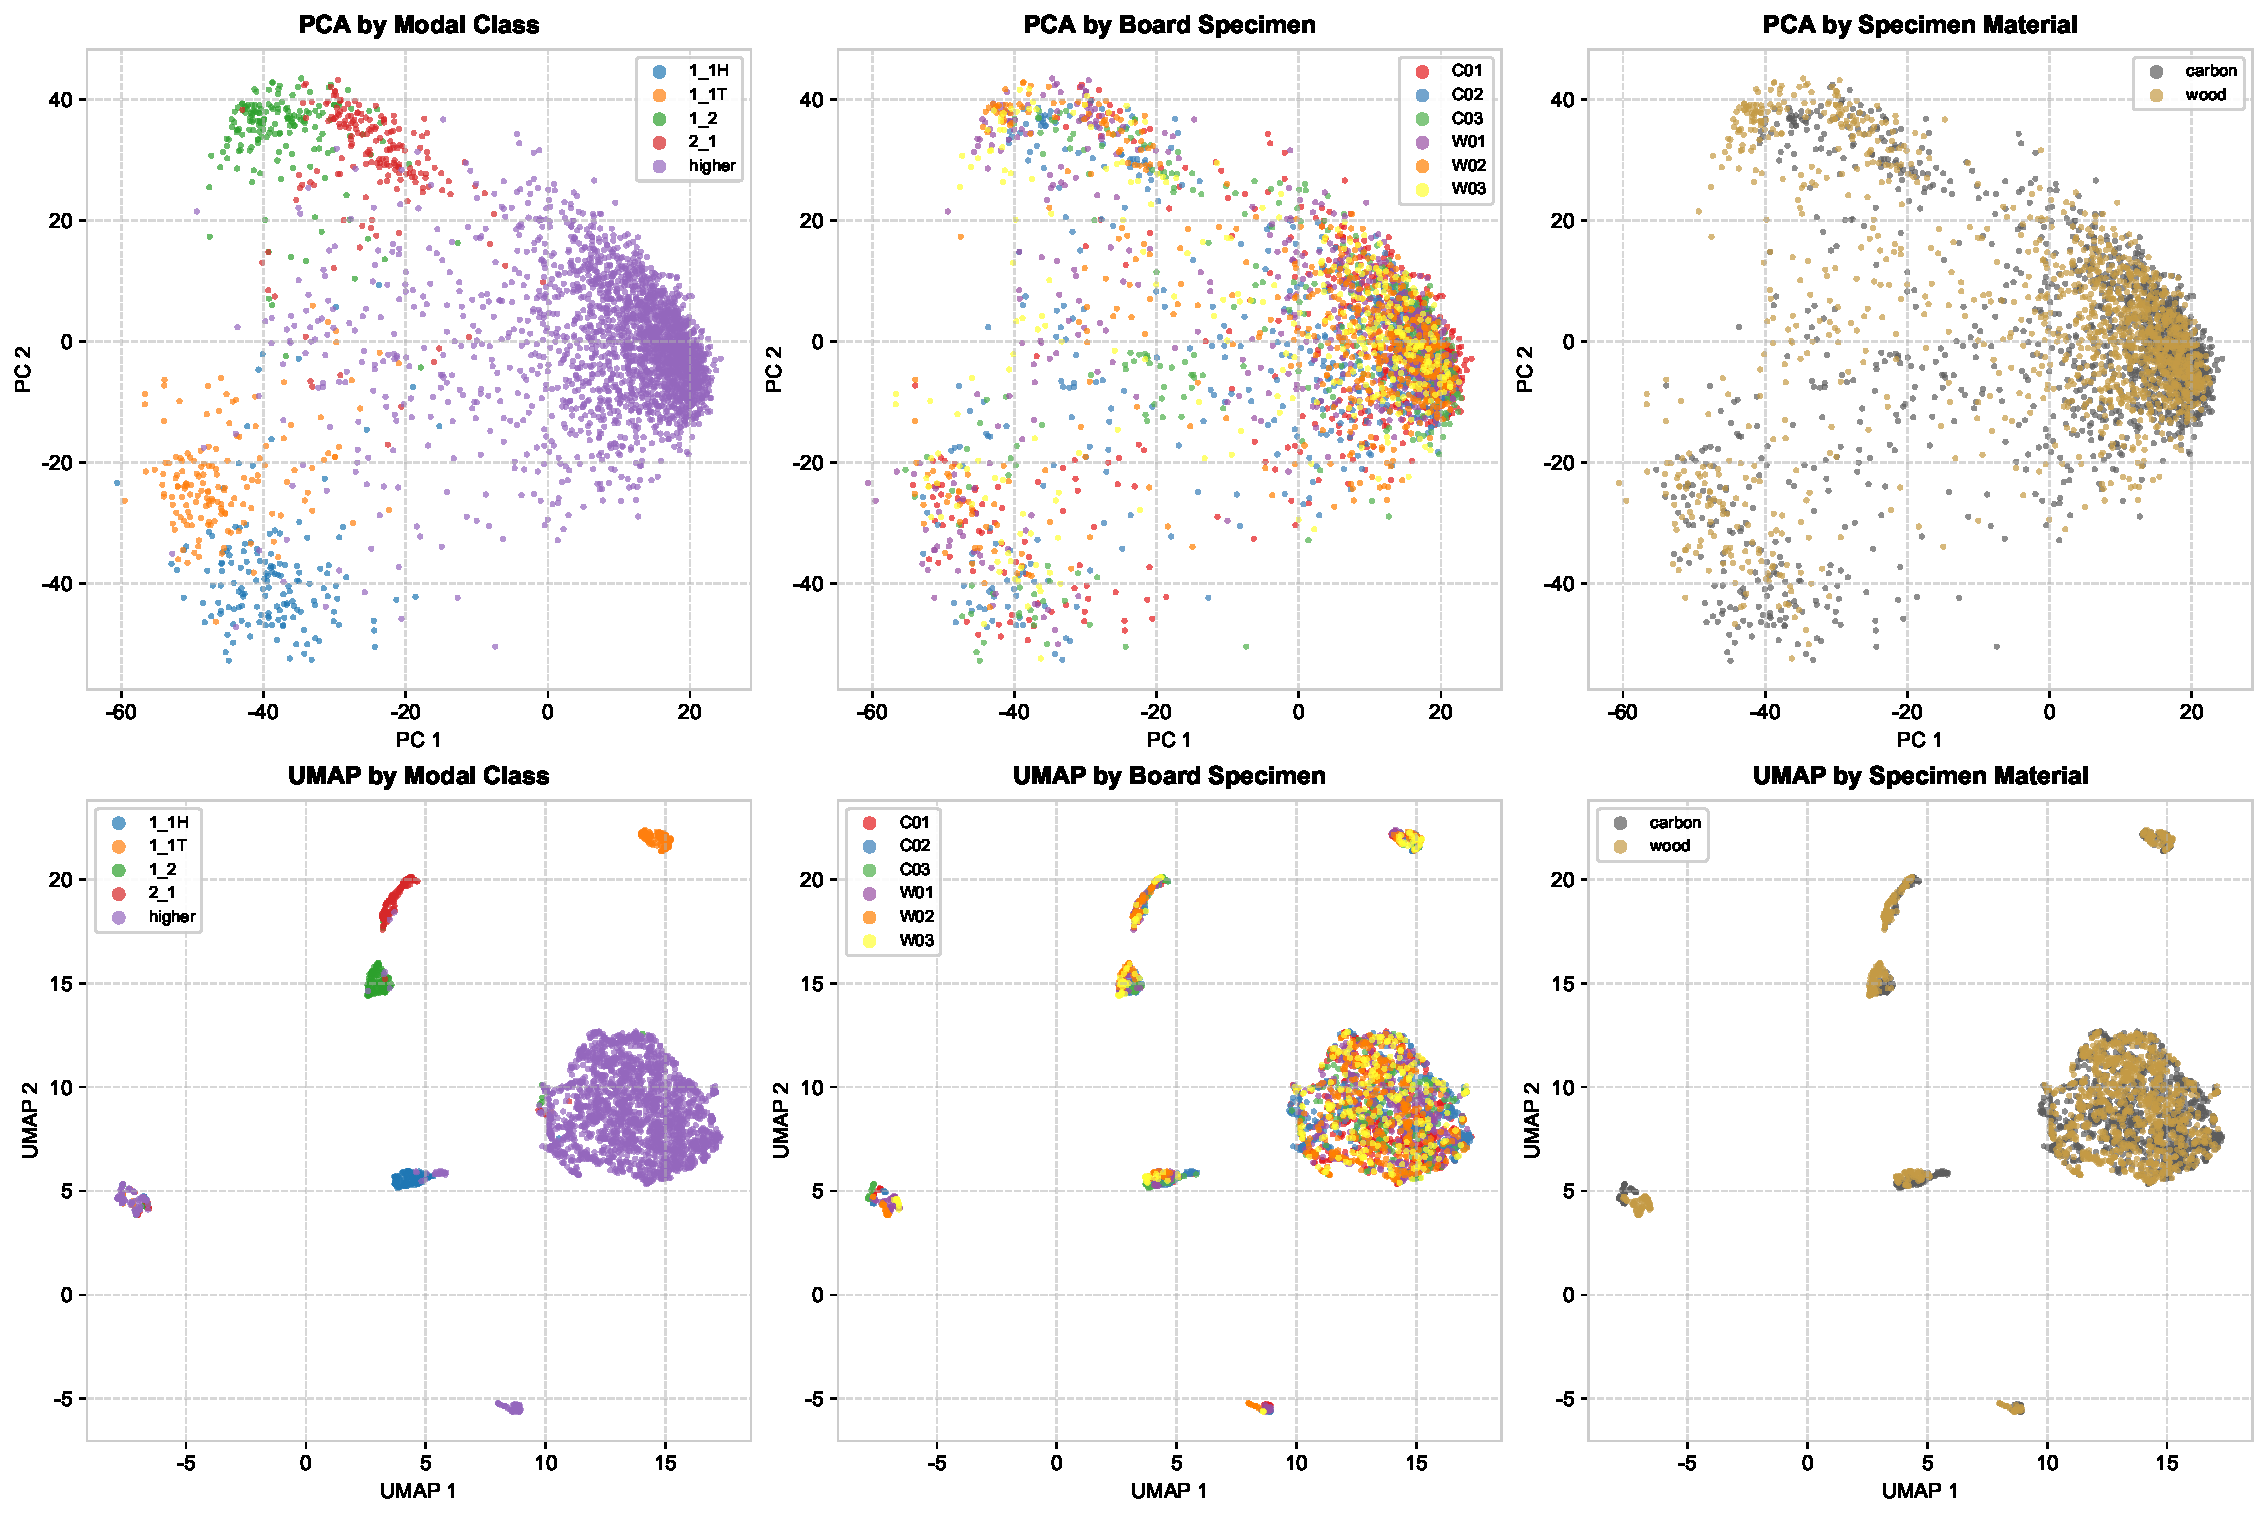
\includegraphics[width=\textwidth]{Figure_PCA_UMAP_Embeddings}
\caption{Dimensionality reduction of frozen v6.2-A representation spaces. Projections under Principal Component Analysis (PCA, top row) and Uniform Manifold Approximation and Projection (UMAP, bottom row), evaluated on a stratified subset of 3,000 samples. The embeddings are color-coded by modal class (left column), board specimen (middle column), and specimen material (right column). The projections qualitatively illustrate class separation and board/material mixing in the v6.2-A representation space. Quantitative geometry metrics are reported separately.}
\label{fig:fig2}
\end{figure}

\begin{table}[htbp]
\centering
\caption{Encoder baseline summary under primary fixed $k=10$ kNN evaluation.}
\label{tab:table1}
\begin{tabular}{lccccc}
\toprule
\textbf{Encoder} & \textbf{Embedding Dim} & \textbf{Stratified F1} & \textbf{Board LOBO F1} & \textbf{Material LOMO F1} \\
\midrule
Random ResNet-18 & 512 & 81.14\% & 26.17\% & 24.59\% \\
ImageNet ResNet-18 & 512 & 84.34\% & 39.30\% & 22.52\% \\
v6.1 Reference Baseline & 512 & \textbf{93.65\%} & 87.10\% & 86.33\% \\
v6.2-A Frozen Encoder & 1280 & 92.78\% & \textbf{93.56\%} & \textbf{93.49\%} \\
Hierarchical v6.2 & 512 & 37.80\% & 24.99\% & 24.47\% \\
\bottomrule
\end{tabular}
\end{table}

\subsection{Stratified Representation Performance}
Under the primary fixed $k=10$ protocol, v6.1 reaches 93.65\% stratified kNN Macro-F1, and v6.2-A reaches 92.78\%. Random ResNet-18, ImageNet ResNet-18, and hierarchical v6.2 phase2 reach 81.14\%, 84.34\%, and 37.80\%, respectively.
The best-k diagnostic does not change the qualitative interpretation. v6.1 reaches 95.07\% at $k=5$, whereas v6.2-A reaches 92.78\% at $k=10$. Best-k values are reported as sensitivity analysis only; fixed $k=10$ is the primary kNN protocol (\cref{tab:table8}).

\subsection{Board-Grouped Robustness}
The board-grouped protocol separates stratified embedding geometry from grouped robustness. At fixed $k=10$, v6.2-A achieves 93.56\% Board LOBO Macro-F1, with a 95\% confidence interval of [92.36\%, 94.67\%]. v6.1 reaches 87.10\%, with a 95\% confidence interval of [82.73\%, 91.23\%] (\cref{tab:table2}). Random ResNet-18 and ImageNet ResNet-18 reach 26.17\% and 39.30\% under their best grouped evaluation methods, while hierarchical v6.2 phase2 reaches 24.99\%.

Paired fold-level comparison shows that v6.2-A improves over v6.1 by +6.47 percentage points in mean Board LOBO Macro-F1 and wins 5/6 board folds. The C02 board is essentially tied (-0.02 pp for v6.2-A relative to v6.1), and W01 shows a small v6.2-A margin (+0.27 pp). The largest board gains occur for C01, W02, and W03 (detailed paired fold-level metrics are provided in Supplementary Table S3).
These results show that v6.2-A preserves class-relevant image-derived structure more effectively when the reference set excludes a board group. A directional paired Wilcoxon signed-rank test over the six Board LOBO folds supported the v6.2-A improvement over v6.1 ($p=0.03125$), with a mean paired gain of +6.47 percentage points and a bootstrap 95\% confidence interval of [+2.09, +10.15] percentage points. Because the number of board folds is small, this test is interpreted together with the fold-level wins, effect size, and bootstrap interval. The collapse of Random and ImageNet controls under board grouping indicates that stratified texture similarity alone is insufficient for board-level ESPI representation robustness.

\begin{table}[htbp]
\centering
\caption{Grouped robustness summary with 95\% bootstrap confidence intervals.}
\label{tab:table2}
\begin{tabular}{lcccc}
\toprule
\textbf{Encoder} & \textbf{Board LOBO F1} & \textbf{Board LOBO 95\% CI} & \textbf{Material LOMO F1} & \textbf{Material LOMO 95\% CI} \\
\midrule
Random ResNet-18 & 26.17\% & N/A & 24.59\% & N/A \\
ImageNet ResNet-18 & 39.30\% & [33.16\%, 46.36\%] & 22.52\% & N/A \\
v6.1 Baseline & 87.10\% & [82.73\%, 91.23\%] & 86.33\% & [85.32\%, 87.34\%] \\
v6.2-A Encoder & \textbf{93.56\%} & [92.36\%, 94.67\%] & \textbf{93.49\%} & [93.01\%, 93.97\%] \\
Hierarchical v6.2 & 24.99\% & N/A & 24.47\% & [23.23\%, 25.71\%] \\
\bottomrule
\end{tabular}
\end{table}

\subsection{Material-Grouped Robustness}
The material-grouped protocol gives the same image-derived encoder conclusion, with the required caution that only two material groups are available. At fixed $k=10$, v6.2-A reaches 93.49\% Material LOMO Macro-F1, with a 95\% confidence interval of [93.01\%, 93.97\%]. v6.1 reaches 86.33\%, with a 95\% confidence interval of [85.32\%, 87.34\%]. Random ResNet-18, ImageNet ResNet-18, and hierarchical v6.2 phase2 reach 24.59\%, 22.52\%, and 24.47\%, respectively.

Paired fold-level comparison shows that v6.2-A improves over v6.1 by +7.16 percentage points in mean Material LOMO Macro-F1 and wins 2/2 material folds (see Supplementary Table S3 for fold-level details). Because the material grouping contains only \texttt{carbon} and \texttt{wood}, this result is interpreted as a descriptive material-held-out stress test rather than as a broad inferential estimate of material generalization.

\subsection{Frequency-only and Frequency-fusion Controls}
Frequency-only controls show that the current modal-label protocol is strongly frequency-structured. Using \texttt{frequency\_hz} as the only input feature, the best frequency-only models reach 98.67\% stratified Macro-F1, 97.49\% Board LOBO Macro-F1, and 94.09\% Material LOMO Macro-F1. These values exceed the image-derived frozen embeddings for the current label task.

Frequency + v6.2-A fusion reaches 96.75\% stratified Macro-F1, 94.79\% Board LOBO Macro-F1, and 94.50\% Material LOMO Macro-F1 (\cref{tab:table7}). Under matched lightweight-head conditions, v6.2-A embedding-only reaches 93.48\%, 94.28\%, and 94.05\% under the same protocols. Frequency + v6.2-A therefore improves over v6.2-A embedding-only by +3.27 pp stratified, +0.50 pp Board LOBO, and +0.45 pp Material LOMO.

\begin{table}[htbp]
\centering
\caption{Frequency-only and frequency+embedding information-budget comparison.}
\label{tab:table7}
\begin{tabular}{lccc}
\toprule
\textbf{Condition} & \textbf{Stratified Macro-F1} & \textbf{Board LOBO Macro-F1} & \textbf{Material LOMO Macro-F1} \\
\midrule
Frequency-only & \textbf{98.67\%} & \textbf{97.49\%} & 94.09\% \\
v6.2-A Embedding-only & 93.48\% & 94.28\% & 94.05\% \\
Frequency + v6.2-A Fusion & 96.75\% & 94.79\% & \textbf{94.50\%} \\
\bottomrule
\end{tabular}
\end{table}

\subsection{Dimension-Matched PCA Control}
To address the concern that the performance advantage of v6.2-A (1280 dimensions) over v6.1 (512 dimensions) is merely an artifact of a larger embedding capacity, we evaluated v6.2-A under dimensionality reduction. A fold-local Principal Component Analysis (PCA) was fitted on each training fold and applied to the corresponding held-out fold to project the 1280-dimensional embeddings down to 512, 256, and 128 dimensions. Under the fixed $k=10$ Board LOBO protocol, the dimension-reduced v6.2-A representations achieve 93.58\% (512 dims), 93.59\% (256 dims), and 93.65\% (128 dims) Macro-F1. Under the Material LOMO protocol, the representations achieve 93.51\% (512 dims), 93.49\% (256 dims), and 93.51\% (128 dims) Macro-F1. These results indicate that the grouped robustness advantage of v6.2-A is not explained solely by the larger 1280-dimensional embedding space.

\begin{table}[htbp]
\centering
\caption{PCA dimension-matched grouped robustness evaluation for v6.2-A representations.}
\label{tab:pca_dimensions}
\begin{tabular}{lcccc}
\toprule
\textbf{Protocol} & \textbf{Original (1280 dims)} & \textbf{PCA (512 dims)} & \textbf{PCA (256 dims)} & \textbf{PCA (128 dims)} \\
\midrule
Board LOBO Macro-F1 & 93.56\% & 93.58\% & 93.59\% & 93.65\% \\
Material LOMO Macro-F1 & 93.49\% & 93.51\% & 93.49\% & 93.51\% \\
\bottomrule
\end{tabular}
\end{table}

\subsection{Targeted Frequency-Overlap Analysis}
To test whether the image-derived representation contributes information beyond scalar excitation frequency in a localized ambiguous regime, we isolated the two structurally similar minority modes \texttt{1\_2} and \texttt{2\_1}. Across the full binary subset ($N=1{,}507$), frequency + v6.2-A fusion substantially improved over the frequency-only baseline. Under Material LOMO, balanced logistic regression increased Macro-F1 from 85.67\% to 96.81\% (+11.14 pp), while a random forest head increased Macro-F1 from 85.67\% to 94.76\% (+9.09 pp). Under Board LOBO, balanced logistic regression increased Macro-F1 from 94.56\% to 98.01\% (+3.45 pp) and random forest increased Macro-F1 from 92.68\% to 96.02\% (+3.34 pp).

We further restricted the evaluation to the narrow frequency-overlap interval from 550.00 to 556.00 Hz ($N=43$), where scalar frequency becomes weakly discriminative. In this subset, the frequency-only logistic-regression baseline reached 52.85\% Macro-F1, whereas the v6.2-A embedding-only and frequency + v6.2-A fusion conditions reached 97.65\% Macro-F1 (bootstrap 95\% CI: [88.37\%, 100.00\%]) (see \cref{tab:table_overlap}). Because the strict overlap subset contains 43 samples, this result is interpreted as a targeted diagnostic of the localized ambiguity rather than as a standalone population-level estimate. This targeted result supports the interpretation that the v6.2-A embedding captures image-derived spatial morphology that resolves the localized frequency ambiguity between \texttt{1\_2} and \texttt{2\_1}.

\begin{table}[htbp]
\centering
\caption{Targeted frequency-overlap and binary classification performance for \texttt{1\_2} vs \texttt{2\_1}.}
\label{tab:table_overlap}
\begin{tabular}{lccccc}
\toprule
\textbf{Subset / Condition} & \textbf{Protocol} & \textbf{Classifier} & \textbf{Frequency-only} & \textbf{v6.2-A embedding-only} & \textbf{Frequency + v6.2-A Fusion} \\
\midrule
\texttt{1\_2}/\texttt{2\_1} binary subset & Material LOMO & LR & 85.67\% & 93.82\% & \textbf{96.81\%} \\
\texttt{1\_2}/\texttt{2\_1} binary subset & Material LOMO & RF & 85.67\% & 93.96\% & \textbf{94.76\%} \\
\texttt{1\_2}/\texttt{2\_1} binary subset & Board LOBO & LR & 94.56\% & 92.56\% & \textbf{98.01\%} \\
\texttt{1\_2}/\texttt{2\_1} binary subset & Board LOBO & RF & 92.68\% & 95.02\% & \textbf{96.02\%} \\
Strict overlap (550--556 Hz) & Stratified & LR & 52.85\% & \textbf{97.65\%} & \textbf{97.65\%} \\
\bottomrule
\end{tabular}
\end{table}

\subsection{Class Support and Imbalance}
The dataset is strongly imbalanced. The \texttt{higher} class contains 10,115 of 12,944 samples, corresponding to 78.14\% of the dataset (Supplementary Table S1). The remaining classes contain 653 samples for \texttt{1\_1H}, 669 for \texttt{1\_1T}, 738 for \texttt{1\_2}, and 769 for \texttt{2\_1}. This imbalance makes class-level diagnostics essential. Macro-F1 reduces majority-class dominance, but per-class analysis is required to determine whether grouped robustness is distributed across modal classes.



\subsection{Per-Class Grouped Stability}
v6.2-A improves grouped F1 over v6.1 across all five modal classes (Supplementary Table S2). The largest gains occur in the difficult minority modal classes. For \texttt{2\_1}, grouped F1 increases from 77.88\% to 91.32\%, a gain of +13.43 percentage points. For \texttt{1\_2}, grouped F1 increases from 78.35\% to 90.57\%, a gain of +12.21 percentage points.
The other classes also improve: \texttt{1\_1H} increases by +3.53 percentage points, \texttt{1\_1T} by +1.49 percentage points, and \texttt{higher} by +0.63 percentage points. The grouped advantage of v6.2-A is therefore visible both in aggregate Macro-F1 and in class-level stability.

\begin{figure}[tbp]
\centering
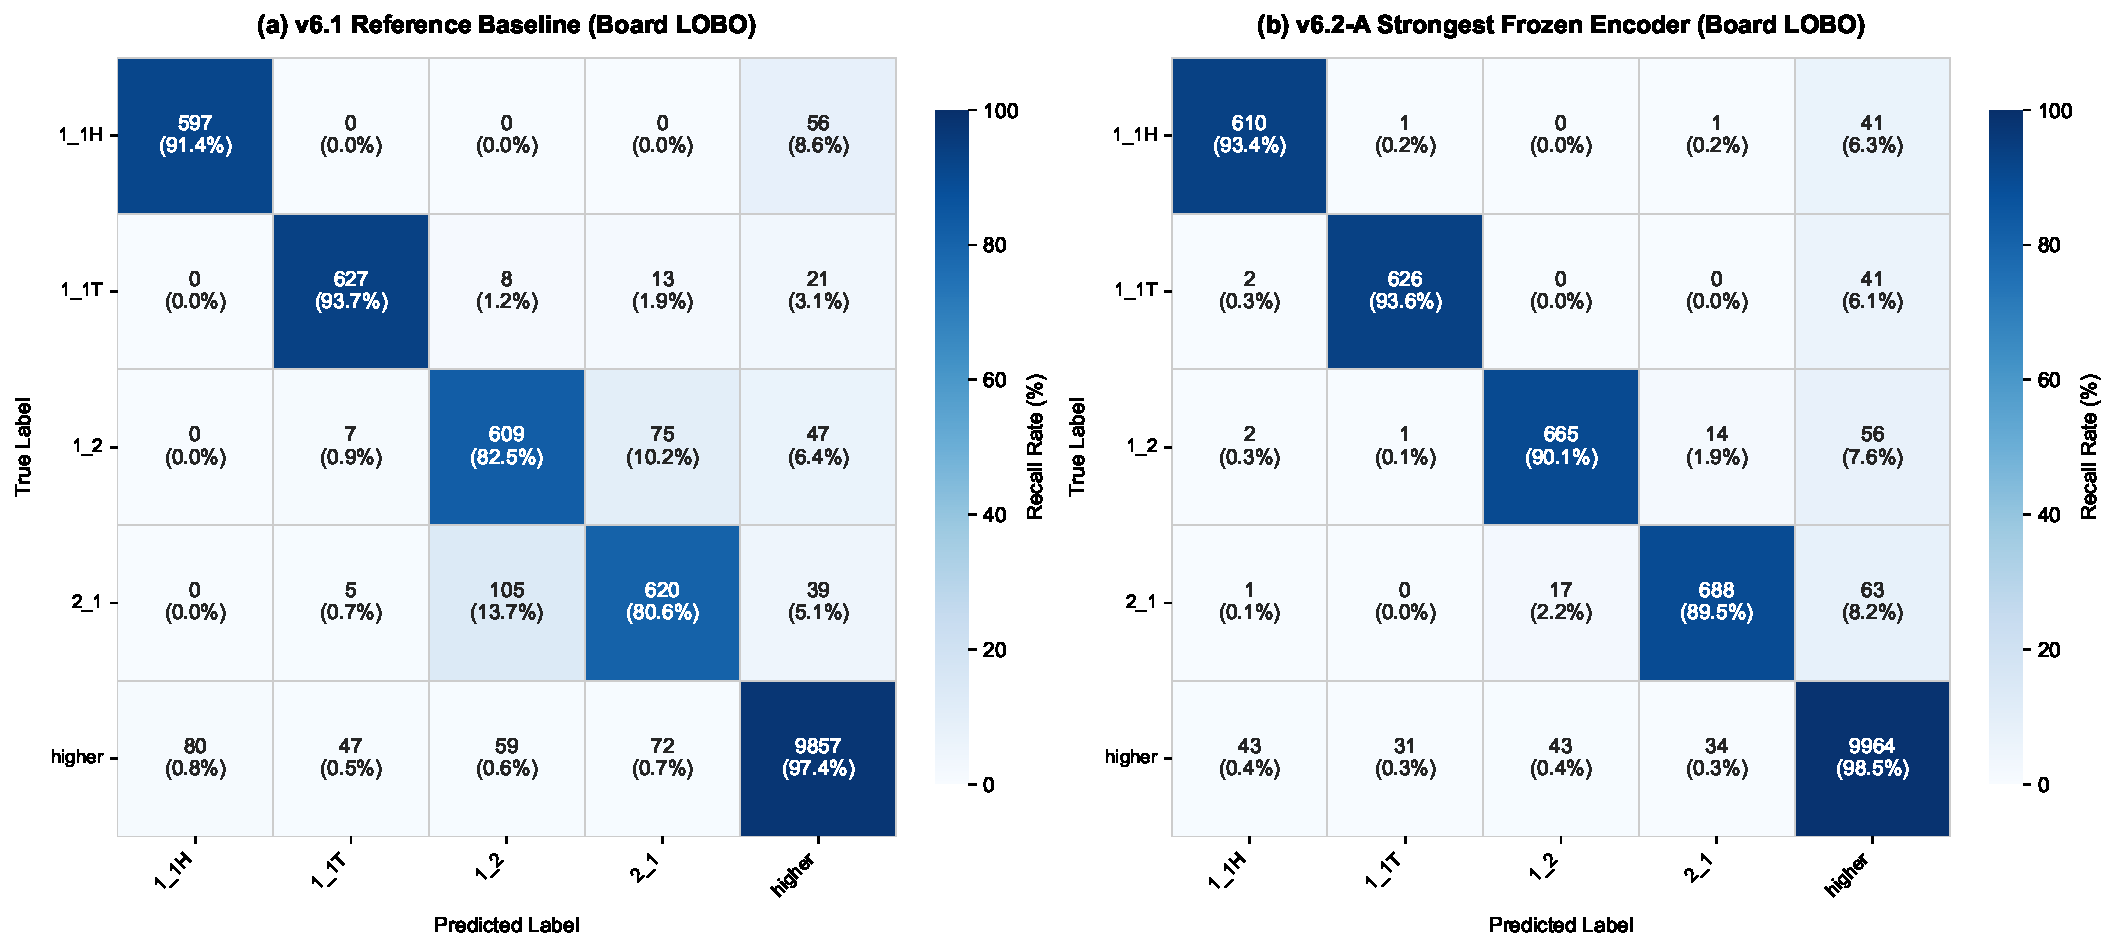
\includegraphics[width=\textwidth]{Figure_Confusion_Matrices_Board_LOBO}
\caption{Side-by-side pooled confusion matrices under Board LOBO protocol. Comparison between (a) the v6.1 reference baseline and (b) the distribution-aware v6.2-A frozen encoder, evaluated using cosine kNN ($k=10$) over all six held-out board folds. Matrix entries report raw sample counts and row-normalized recall percentages. The comparison highlights the major suppression of cross-class confusion between the structurally similar minority modes 1\_2 and 2\_1, dropping from 13.7\% to 2.2\% (for true 2\_1 predicted as 1\_2) and from 10.2\% to 1.9\% (for true 1\_2 predicted as 2\_1), respectively.}
\label{fig:fig3}
\end{figure}


\subsection{Zero-Recall Analysis}
Zero-recall failures are concentrated in the generic and hierarchical baselines. The generated summary reports 20 zero-recall rows for ImageNet ResNet-18, 18 for Random ResNet-18, and 9 for hierarchical v6.2 phase2 (Supplementary Table S3). No zero-recall rows are attributed to v6.1 or v6.2-A in the generated summary.
This pattern shows that grouped failures in the weaker baselines include complete class-level failures in specific grouped conditions. v6.1 and v6.2-A avoid zero-recall rows in the generated diagnostic summary, with v6.2-A additionally providing higher grouped per-class F1 across all classes.



\subsection{Balanced Subset Robustness Analysis}
To test whether the grouped robustness advantage of v6.2-A is driven by class imbalance, material imbalance, or frequency-distribution artifacts, we repeated the frozen-embedding evaluation on three balanced subsets: class-balanced, class--material-balanced, and class--material--frequency-matched. The strictest subset matched wood and carbon samples within 25 Hz frequency bins inside each modal class and then applied final class balancing, yielding 184 samples per class and 920 samples in total.

The grouped advantage of v6.2-A persisted across all balanced subset conditions (\cref{tab:balanced_subset}). In the strictest class--material--frequency-matched subset, v6.2-A achieved 94.83\% Board LOBO Macro-F1, compared with 86.43\% for v6.1, corresponding to a +8.40 percentage-point gain. Under Material LOMO, v6.2-A achieved 94.73\% Macro-F1, compared with 81.81\% for v6.1, corresponding to a +12.92 percentage-point gain. These results support the interpretation that the grouped robustness advantage of v6.2-A persists after controlling for the main dataset-structure confounders: class imbalance, material composition, and frequency-bin distribution.

\begin{table}[htbp]
\centering
\caption{Balanced subset grouped evaluation. Macro-F1 is reported for v6.1 and v6.2-A under class-balanced, class--material-balanced, and class--material--frequency-matched subsets.}
\label{tab:balanced_subset}
\begin{tabular}{llccc}
\toprule
\textbf{Subset} & \textbf{Protocol} & \textbf{v6.1} & \textbf{v6.2-A} & \textbf{$\Delta$ (pp)} \\
\midrule
Class-balanced & Board LOBO & 90.23\% & 94.42\% & +4.19 pp \\
Class-balanced & Material LOMO & 88.64\% & 93.64\% & +5.00 pp \\
Class--material-balanced & Board LOBO & 89.89\% & 93.86\% & +3.97 pp \\
Class--material-balanced & Material LOMO & 88.24\% & 93.73\% & +5.49 pp \\
Class--material--frequency-matched & Board LOBO & 86.43\% & 94.83\% & +8.40 pp \\
Class--material--frequency-matched & Material LOMO & 81.81\% & 94.73\% & +12.92 pp \\
\bottomrule
\end{tabular}
\end{table}



\subsection{Quantitative Embedding Geometry and Nearest-Neighbor Consistency}
To complement the downstream kNN and grouped evaluation results, we directly quantified the geometry of the frozen embedding spaces. Compared with v6.1, v6.2-A achieved a higher cosine Silhouette score (0.7248 versus 0.5789), a lower Davies--Bouldin index (0.6453 versus 1.0540), and a lower intra/inter-class cosine distance ratio (0.1698 versus 0.3230). These results indicate tighter within-class structure and stronger between-class separation in the v6.2-A representation space.

Nearest-neighbor consistency also improved under grouped conditions (\cref{tab:embedding_geometry}). The cross-board same-class nearest-neighbor rate increased from 95.37\% for v6.1 to 96.38\% for v6.2-A, and the cross-material same-class nearest-neighbor rate increased from 94.21\% to 96.52\%. The per-class intra/inter distance analysis showed improvements across all five modal classes, with the largest reductions for the frequency-overlapping minority modes \texttt{1\_2} and \texttt{2\_1} (see \cref{tab:per_class_geometry} in the appendix). These findings support the interpretation that the grouped robustness of v6.2-A is reflected in the geometry of the frozen representation space, not only in the downstream classifier metrics.

\begin{table}[htbp]
\centering
\caption{Quantitative frozen-embedding geometry comparison between v6.1 and v6.2-A. Higher Silhouette and nearest-neighbor consistency are better; lower Davies--Bouldin and intra/inter distance ratio are better.}
\label{tab:embedding_geometry}
\begin{tabular}{lccc}
\toprule
\textbf{Metric} & \textbf{v6.1} & \textbf{v6.2-A} & \textbf{Direction} \\
\midrule
Cosine Silhouette score & 0.5789 & 0.7248 & $\uparrow$ \\
Davies--Bouldin index & 1.0540 & 0.6453 & $\downarrow$ \\
Intra/inter cosine distance ratio & 0.3230 & 0.1698 & $\downarrow$ \\
Cross-board same-class NN rate & 95.37\% & 96.38\% & $\uparrow$ \\
Cross-material same-class NN rate & 94.21\% & 96.52\% & $\uparrow$ \\
\bottomrule
\end{tabular}
\end{table}



\subsection{Controlled Hierarchical Comparison}
Hierarchical v6.2 phase2 provides a controlled physics-aware architecture comparison (Supplementary Table S8). The checkpoint is technically valid and produces frozen embeddings, but it is not superior in this representation evaluation. It reaches 37.80\% stratified kNN Macro-F1, 24.99\% Board LOBO Macro-F1, and 24.47\% Material LOMO Macro-F1.

This result should be interpreted at the checkpoint and representation-evaluation level. Architecture-level physics-aware components do not automatically imply robust post-hoc embedding geometry. The resulting decision flow selects v6.2-A as the primary reportable image-derived frozen ESPI encoder baseline, retains v6.1 as the strongest stratified image-derived reference, and keeps hierarchical v6.2 phase2 as a controlled physics-aware alternative rather than a final validated encoder.

\section{Discussion}
\label{sec:discussion}

\subsection{Grouped Robustness Rather than Overall Predictive Dominance}
The central image-derived representation result is the distinction between stratified embedding geometry and grouped board/material robustness. Under fixed $k=10$, v6.1 is slightly stronger in stratified kNN Macro-F1 (93.65\%) than v6.2-A (92.78\%). Under grouped fixed $k=10$ evaluation, v6.2-A is strongest among image-derived encoders, reaching 93.56\% Board LOBO Macro-F1 and 93.49\% Material LOMO Macro-F1.

The frequency controls define the information budget of the present label protocol. Frequency metadata is a stronger overall predictor than any image-derived frozen representation for this five-class task. This refines the representation claim rather than weakening it: the encoder comparison concerns image-derived representations under matched grouped protocols, where v6.2-A remains the strongest image-derived baseline. Demonstrating image-derived information beyond modal frequency structure will require frequency-controlled labels, frequency-residual prediction, or acoustic-response targets.

This frequency dominance is further refined by our targeted localized analysis of structurally similar and frequency-overlapping modes. While frequency metadata dominates the global five-class label protocol, v6.2-A embeddings provide complementary image-derived morphology in the physically ambiguous \texttt{1\_2} / \texttt{2\_1} frequency-overlap region. In this specific frequency band (550.00 to 556.00 Hz), the two modes occupy highly overlapping excitation ranges, where scalar frequency becomes weakly discriminative. However, the image-derived v6.2-A representation provides spatial fringe-morphology information that helps separate the two modes. These results support the interpretation that the v6.2-A embedding captures image-derived spatial morphology that resolves the localized frequency ambiguity between \texttt{1\_2} and \texttt{2\_1}, demonstrating that the visual fringe morphology encodes structural information that complements the excitation frequency when the latter is ambiguous.

The balanced subset analysis further strengthens this interpretation. When the evaluation is repeated under class-balanced, class--material-balanced, and class--material--frequency-matched sampling, v6.2-A retains its grouped advantage over v6.1. In the strictest frequency-matched balanced subset, the gain reaches +8.40 percentage points under Board LOBO and +12.92 percentage points under Material LOMO. This indicates that the grouped robustness result is not explained by the dominant \texttt{higher} class, by unequal material support, or by frequency-bin distribution differences alone.

The embedding-geometry diagnostics provide an independent representation-level explanation for the grouped results. v6.2-A improves the global Silhouette score, reduces the Davies--Bouldin index, and nearly halves the intra/inter-class cosine distance ratio relative to v6.1. The largest per-class reductions occur for \texttt{1\_2} and \texttt{2\_1}, the same frequency-overlapping minority modes identified in the targeted residual analysis. This alignment between grouped performance, frequency-overlap correction, and embedding geometry supports the interpretation that v6.2-A learns a more compact and class-consistent image-derived representation.

\subsection{Why Grouped Evaluation Matters for ESPI Representations}
ESPI images preserve full-field interferometric structure, but this structure can include signatures associated with board geometry, material, acquisition condition, and frequency sampling. Stratified validation may overestimate representation robustness if related samples share these signatures across train and validation splits.

Grouped board/material evaluation provides a stricter representation-level test. The board-grouped protocol excludes the held-out board from the reference set; the material-grouped protocol excludes the held-out material. These tests evaluate whether a fixed embedding space remains useful under grouped distribution-shift conditions. The grouped performance of v6.2-A therefore supports its use as a frozen image-derived ESPI encoder baseline for transferable representation studies.

\subsection{Per-Class Grouped Stability}
The class-level diagnostics show that the grouped advantage of v6.2-A is not only an aggregate effect. v6.2-A improves grouped F1 over v6.1 across all five modal classes, with the largest gains in \texttt{2\_1} (+13.43 percentage points) and \texttt{1\_2} (+12.21 percentage points).

This is important because the dataset is dominated by the \texttt{higher} class, which contributes 10,115 samples, or 78.14\% of the dataset. If the grouped gain were driven only by the majority class, it would be less informative as encoder evidence. Instead, the largest gains occur in minority modal classes, indicating improved grouped class stability. The substantially lower prototype performance (70.97\%) relative to kNN (93.56\%) under Board LOBO (see \cref{tab:downstream_heads} in the appendix) indicates that each modal class spans multiple board/material submanifolds in the embedding space, and a single class centroid is insufficient to capture this multimodal structure.

\subsection{Interpretation of Generic and Spectral Controls}
Random and ImageNet ResNet-18 baselines show non-trivial stratified Macro-F1 but collapse under grouped evaluation. This indicates that generic texture features can support stratified separability when train and validation samples share acquisition or grouping structure, but do not provide stable grouped ESPI representations.

Deterministic FFT-based descriptors were evaluated as a supplementary spectral control. Their weak grouped performance indicates that simple handcrafted spatial-frequency summaries do not explain the grouped robustness achieved by v6.2-A. Detailed performance metrics for these supplementary controls are available in Supplementary Table S4.

\subsection{Interpretation of Hierarchical v6.2 Phase2}
Hierarchical v6.2 phase2 is technically valid but not superior in this frozen embedding evaluation. It provides a controlled physics-aware architectural comparison, but its frozen embeddings do not outperform v6.2-A under stratified, board-grouped, or material-grouped evaluation.

This result shows that physics-aware architecture alone does not guarantee robust frozen embedding geometry. A representation-aligned training objective, contrastive fine-tuning, or a different extraction point may be required before the hierarchical branch can serve as a stronger encoder candidate. The result should not be interpreted as a LeFFT failure; learned spectral modules and LeFFT-style architectures remain future work requiring matched ablation.

\section{Limitations and Future Work}
\label{sec:limitations}

This study evaluates frozen embeddings rather than CNNs retrained under full LOBO/LOMO protocols. The grouped board/material tests change the reference and held-out groups while keeping encoder weights fixed. The results support frozen grouped representation evidence, not retrained CNN grouped generalization.

Frequency metadata dominates the current five-class modal-label protocol. Frequency-only controls exceed the image-derived embeddings for the present label task, so v6.2-A is not the strongest overall predictor when metadata is allowed. The image-derived frozen encoder claim is specifically about representation quality among frozen ESPI image encoders under matched grouped protocols.

Material LOMO uses only two material groups (\texttt{carbon} and \texttt{wood}) and is interpreted as a descriptive material-held-out stress test.

The study does not evaluate acoustic-response prediction. It does not test whether ESPI embeddings improve prediction of acoustic, phononic, or metamaterial response variables. Such prediction requires separate targets, baselines, and information-budget controls.

The study also does not establish a complete physics-aligned encoder. v6.2-A is identified as the primary reportable image-derived frozen ESPI encoder baseline for grouped representation studies, but further validation would be required before claiming a fully physics-aligned representation.

The hierarchical v6.2 phase2 feature dump provides a valid representation for a controlled physics-aware architecture comparison. While future validation should include direct integration of board and split-group metadata in the source feature dump, this does not affect its current evaluation as an architecture control, nor does it impact the primary v6.2-A conclusion.

Deterministic spectral / LeFFT-inspired descriptors were evaluated as a supplementary control. Spectral-only descriptors were not competitive, and adding spectral descriptors to frequency + v6.2-A yielded only marginal grouped gains. No LeFFT superiority claim is supported. Learned spectral modules or LeFFT-style architectures remain future work.

Representation-aligned fine-tuning is another natural next step. Supervised contrastive learning, triplet objectives, or domain-aware batch construction could encourage same-mode samples from different boards or materials to occupy nearby regions of the embedding space while preserving class separation.

Future work should explicitly test image-derived information beyond frequency structure. Suitable protocols include frequency-controlled labels, frequency-residual prediction, acoustic-response targets, or tasks where image-derived morphology must explain variance beyond modal frequency metadata. Only after such validation should downstream use in acoustic or phononic systems be claimed.

\section{Conclusion}
\label{sec:conclusion}

This study audits frozen ESPI representation spaces under fixed stratified and grouped protocols. v6.1 remains slightly stronger under fixed $k=10$ stratified kNN, indicating strong in-distribution embedding geometry. v6.2-A provides the strongest grouped board/material robustness among the evaluated image-derived frozen encoders.

Class-level diagnostics show that v6.2-A improves grouped F1 across all five modal classes, with the largest gains in the difficult minority classes \texttt{2\_1} and \texttt{1\_2}. Frequency-only and frequency-fusion controls show that the current modal-label protocol is strongly frequency-structured; frequency metadata is a dominant predictor, while frequency + v6.2-A provides limited complementary gains over embedding-only and a small Material LOMO gain over frequency-only.

The work establishes an encoder-evidence stage between ESPI classification and future physically grounded representation learning. It supports frozen grouped image-derived representation evidence while leaving acoustic-response prediction, frequency-controlled tasks, learned spectral ablations, and full encoder validation as future work.


\section*{Data, Code, and Reproducibility Availability}
The analysis is based on frozen feature dumps, normalized metadata schemas, lightweight evaluation scripts, metadata controls, deterministic spectral descriptor controls, and methodological hardening audits. No deep model retraining, acoustic-response prediction, trained LeFFT model, or LeFFT superiority claim is part of the reported results. The reproducibility package should include the normalized frozen feature schema, encoder evaluation scripts, class-level diagnostic scripts, frequency-control scripts, spectral descriptor control scripts, publication tables and figures, claim checklist, and audit reports. Data and code release details should be finalized according to institutional permissions and the target journal's repository policy.

\subsection*{Reproducibility Notes}
The hierarchical v6.2 phase2 feature dump contains embeddings that provide a valid representation for a controlled physics-aware architecture comparison. While future validation should include direct integration of board and split-group metadata in the source feature dump, this does not affect its current evaluation as an architecture control, nor does it impact the primary v6.2-A conclusions.

\section*{References}
\begin{thebibliography}{99}

\bibitem{jones1989} R. Jones and C. Wykes, \emph{Holographic and Speckle Interferometry}, Cambridge University Press, 1989.

\bibitem{rastogi2001} P. K. Rastogi, Ed., \emph{Digital Speckle Pattern Interferometry and Related Techniques}, Wiley, 2001.

\bibitem{takeda1982} M. Takeda, H. Ina, and S. Kobayashi, ``Fourier-transform method of fringe-pattern analysis for computer-based topography and interferometry,'' \emph{Journal of the Optical Society of America}, vol. 72, no. 1, pp. 156-160, 1982. \url{https://doi.org/10.1364/JOSA.72.000156}

\bibitem{ghiglia1998} D. C. Ghiglia and M. D. Pritt, \emph{Two-Dimensional Phase Unwrapping: Theory, Algorithms, and Software}, Wiley, 1998.

\bibitem{goodman2007} J. W. Goodman, \emph{Speckle Phenomena in Optics: Theory and Applications}, Roberts and Company, 2007.

\bibitem{he2016} K. He, X. Zhang, S. Ren, and J. Sun, ``Deep Residual Learning for Image Recognition,'' in \emph{Proceedings of the IEEE Conference on Computer Vision and Pattern Recognition (CVPR)}, pp. 770-778, 2016. \url{https://doi.org/10.1109/CVPR.2016.90}

\bibitem{deng2009} J. Deng, W. Dong, R. Socher, L.-J. Li, K. Li, and L. Fei-Fei, ``ImageNet: A Large-Scale Hierarchical Image Database,'' in \emph{Proceedings of the IEEE Conference on Computer Vision and Pattern Recognition (CVPR)}, pp. 248-255, 2009. \url{https://doi.org/10.1109/CVPR.2009.5206848}

\bibitem{gulrajani2021} I. Gulrajani and D. Lopez-Paz, ``In Search of Lost Domain Generalization,'' in \emph{International Conference on Learning Representations (ICLR)}, 2021.

\bibitem{yan2019} K. Yan, Y. Yu, C. Huang, L. Sui, K. Qian, and A. Anand, ``Fringe pattern denoising based on deep learning,'' \emph{Optics Communications}, vol. 437, pp. 148-152, 2019. \url{https://doi.org/10.1016/j.optcom.2018.12.058}

\bibitem{feng2019} S. Feng, Q. Chen, G. Gu, T. Tao, L. Zhang, Y. Hu, W. Yin, and C. Zuo, ``Fringe pattern analysis using deep learning,'' \emph{Advanced Photonics}, vol. 1, 025001, 2019. \url{https://doi.org/10.1117/1.AP.1.2.025001}

\bibitem{zuo2022} C. Zuo, J. Qian, S. Feng, W. Yin, Y. Li, P. Fan, J. Han, K. Qian, and Q. Chen, ``Deep learning in optical metrology: a review,'' \emph{Light: Science \& Applications}, vol. 11, 39, 2022. \url{https://doi.org/10.1038/s41377-022-00714-x}

\bibitem{wang2019} K. Wang, Y. Li, Q. Kemao, J. Di, and J. Zhao, ``One-step robust deep learning phase unwrapping,'' \emph{Optics Express}, vol. 27, pp. 15100-15115, 2019. \url{https://doi.org/10.1364/OE.27.015100}

\bibitem{sun2021} M. Sun, Z. Zhang, and X. Gao, ``Deep learning-based fringe pattern analysis for optical metrology,'' \emph{Measurement Science and Technology}, vol. 32, 112001, 2021. \url{https://doi.org/10.1088/1361-6501/ac0b4e}

\bibitem{bengio2013} Y. Bengio, A. Courville, and P. Vincent, ``Representation learning: A review and new perspectives,'' \emph{IEEE Transactions on Pattern Analysis and Machine Intelligence}, vol. 35, pp. 1798-1828, 2013. \url{https://doi.org/10.1109/TPAMI.2013.50}

\end{thebibliography}

\appendix
\section{Supplementary Tables}
\label{sec:appendix}

\renewcommand{\thetable}{S\arabic{table}}
\setcounter{table}{0}

\begin{table}[htbp]
\centering
\caption{Class support and dataset imbalance.}
\label{tab:table4}
\begin{tabular}{ccccc}
\toprule
\textbf{Class ID} & \textbf{Class Name} & \textbf{Total Support} & \textbf{Support (\%)} & \textbf{Imbalance Notes} \\
\midrule
0 & \texttt{1\_1H} & 653 & 5.04\% & Minority class; highly sensitive to errors. \\
1 & \texttt{1\_1T} & 669 & 5.17\% & Minority class; highly sensitive to errors. \\
2 & \texttt{1\_2} & 738 & 5.70\% & Minority class; highly sensitive to errors. \\
3 & \texttt{2\_1} & 769 & 5.94\% & Minority class; highly sensitive to errors. \\
4 & \texttt{higher} & 10,115 & 78.14\% & Dominant majority class. \\
\bottomrule
\end{tabular}
\end{table}

\begin{table}[htbp]
\centering
\caption{v6.2-A vs v6.1 per-class grouped stability comparison.}
\label{tab:table5}
\begin{tabular}{lcccc}
\toprule
\textbf{Class Name} & \textbf{v6.1 Grouped F1} & \textbf{v6.2-A Grouped F1} & \textbf{Delta (pp)} & \textbf{Interpretation} \\
\midrule
\texttt{2\_1} & 77.88\% & 91.32\% & +13.43 pp & Large grouped stability gain for complex torsional mode. \\
\texttt{1\_2} & 78.35\% & 90.57\% & +12.21 pp & Large grouped stability gain for two-axial bending mode. \\
\texttt{1\_1H} & 89.11\% & 92.65\% & +3.53 pp & Moderate grouped stability gain. \\
\texttt{1\_1T} & 92.97\% & 94.46\% & +1.49 pp & Small positive grouped stability gain. \\
\texttt{higher} & 97.63\% & 98.26\% & +0.63 pp & Small positive grouped stability gain. \\
\bottomrule
\end{tabular}
\end{table}

\begin{table}[htbp]
\centering
\caption{Zero-recall breakdown by encoder under grouped conditions.}
\label{tab:table6}
\begin{tabular}{lccl}
\toprule
\textbf{Encoder} & \textbf{Zero-recall Rows} & \textbf{Affected Conditions} & \textbf{Interpretation} \\
\midrule
Random ResNet-18 & 18 & Board/Material Grouped & Unstable grouped class recovery. \\
ImageNet ResNet-18 & 20 & Board/Material Grouped & Unstable grouped class recovery. \\
v6.1 & 0 & None & Stable grouped class recovery. \\
v6.2-A & 0 & None & Stable grouped class recovery with highest F1. \\
Hierarchical v6.2 & 9 & Board/Material Grouped & Unstable grouped class recovery. \\
\bottomrule
\end{tabular}
\end{table}

\begin{table}[htbp]
\centering
\caption{Board-level support.}
\label{tab:s1}
\begin{tabular}{lcccccc}
\toprule
\textbf{Board} & \texttt{1\_1H} & \texttt{1\_1T} & \texttt{1\_2} & \texttt{2\_1} & \texttt{higher} & \textbf{Total} \\
\midrule
C01 & 109 & 108 & 111 & 114 & 1485 & 1927 \\
C02 & 108 & 110 & 110 & 113 & 1494 & 1935 \\
C03 & 110 & 111 & 112 & 112 & 1478 & 1925 \\
W01 & 108 & 112 & 136 & 142 & 1888 & 2386 \\
W02 & 110 & 114 & 134 & 144 & 1892 & 2394 \\
W03 & 108 & 114 & 135 & 144 & 1878 & 2377 \\
\textbf{Total} & \textbf{653} & \textbf{669} & \textbf{738} & \textbf{769} & \textbf{10115} & \textbf{12944} \\
\bottomrule
\end{tabular}
\end{table}

\begin{table}[htbp]
\centering
\caption{Material-level support.}
\label{tab:s2}
\begin{tabular}{lcccccc}
\toprule
\textbf{Material} & \texttt{1\_1H} & \texttt{1\_1T} & \texttt{1\_2} & \texttt{2\_1} & \texttt{higher} & \textbf{Total} \\
\midrule
carbon & 327 & 329 & 333 & 339 & 4457 & 5785 \\
wood & 326 & 340 & 405 & 430 & 5658 & 7159 \\
\textbf{Total} & \textbf{653} & \textbf{669} & \textbf{738} & \textbf{769} & \textbf{10115} & \textbf{12944} \\
\bottomrule
\end{tabular}
\end{table}

\begin{table}[htbp]
\centering
\caption{Paired board/material deltas (v6.2-A vs v6.1 Macro-F1).}
\label{tab:s5}
\begin{tabular}{lcccc}
\toprule
\textbf{Held-out Fold} & \textbf{v6.1 F1} & \textbf{v6.2-A F1} & \textbf{Delta (pp)} & \textbf{Result} \\
\midrule
Board C01 & 81.38\% & 92.54\% & +11.16 pp & v6.2-A win \\
Board C02 & 93.62\% & 93.60\% & -0.02 pp & Tie / minor delta \\
Board C03 & 88.42\% & 94.12\% & +5.70 pp & v6.2-A win \\
Board W01 & 91.24\% & 91.51\% & +0.27 pp & v6.2-A win \\
Board W02 & 83.42\% & 94.61\% & +11.19 pp & v6.2-A win \\
Board W03 & 84.52\% & 95.01\% & +10.49 pp & v6.2-A win \\
\textbf{Mean Board LOBO} & \textbf{87.10\%} & \textbf{93.56\%} & \textbf{+6.47 pp} & \textbf{v6.2-A win (5/6 folds)} \\
\midrule
Material Carbon $\rightarrow$ Wood & 85.32\% & 93.01\% & +7.69 pp & v6.2-A win \\
Material Wood $\rightarrow$ Carbon & 87.34\% & 93.97\% & +6.63 pp & v6.2-A win \\
\textbf{Mean Material LOMO} & \textbf{86.33\%} & \textbf{93.49\%} & \textbf{+7.16 pp} & \textbf{v6.2-A win (2/2 folds)} \\
\bottomrule
\end{tabular}
\end{table}

\begin{table}[htbp]
\centering
\caption{Deterministic spectral descriptor control. Spectral descriptors are handcrafted FFT-based summaries and are not a trained LeFFT model.}
\label{tab:spectral_control}
\begin{tabular}{lccc}
\toprule
Condition & Stratified Macro-F1 & Board LOBO Macro-F1 & Material LOMO Macro-F1 \\
\midrule
Spectral-only descriptors & 52.92\% & 22.77\% & 19.72\% \\
v6.2-A embedding-only & 93.48\% & 94.28\% & 94.05\% \\
v6.2-A + spectral descriptors & -- & 94.35\% & 94.00\% \\
\bottomrule
\end{tabular}
\end{table}

\begin{table}[htbp]
\centering
\caption{Per-class intra/inter cosine distance ratio. Lower values indicate tighter class structure relative to separation from other classes.}
\label{tab:per_class_geometry}
\begin{tabular}{lccc}
\toprule
\textbf{Class} & \textbf{v6.1} & \textbf{v6.2-A} & \textbf{$\Delta$} \\
\midrule
\texttt{1\_1H} & 0.2293 & 0.1534 & -0.0760 \\
\texttt{1\_1T} & 0.2762 & 0.1554 & -0.1209 \\
\texttt{1\_2} & 0.4326 & 0.1951 & -0.2376 \\
\texttt{2\_1} & 0.3909 & 0.1557 & -0.2352 \\
\texttt{higher} & 0.2858 & 0.1893 & -0.0965 \\
\bottomrule
\end{tabular}
\end{table}

\begin{table}[htbp]
\centering
\caption{Downstream head sensitivity analysis for frozen v6.2-A representation. The table compares F1 performance under different downstream probes across the grouped evaluation protocols.}
\label{tab:downstream_heads}
\begin{tabular}{lccc}
\toprule
\textbf{Protocol} & \textbf{Cosine kNN ($k=10$)} & \textbf{Linear Probe (Logistic Regression)} & \textbf{Nearest Class Prototype} \\
\midrule
Board LOBO Mean & 93.56\% & 91.40\% & 70.97\% \\
Material LOMO Mean & 93.49\% & 91.17\% & 71.35\% \\
\bottomrule
\end{tabular}
\end{table}

\begin{table}[htbp]
\centering
\caption{Controlled architecture and publication decisions.}
\label{tab:table3}
\begin{tabular}{lcccl}
\toprule
\textbf{Encoder} & \textbf{Embedding Point} & \textbf{Stratified F1} & \textbf{Board LOBO F1} & \textbf{Publication Decision} \\
\midrule
v6.1 Reference & \texttt{avgpool\_pre\_classifier} & 93.65\% & 87.10\% & Retain as strongest stratified reference. \\
v6.2-A Encoder & \texttt{MCDropout.global\_pool} & 92.78\% & \textbf{93.56\%} & Use as primary reportable frozen encoder baseline. \\
Hierarchical v6.2 & \texttt{z\_expert\_prelogit} & 37.80\% & 24.99\% & Retain as controlled physics alternative. \\
\bottomrule
\end{tabular}
\end{table}



\end{document}
